\section{Click models}
\begin{itemize}
	\item User clicks can be used as evaluation of IR systems as clicks indicate the relevance of a document
	\item However, clicks are highly biased (positional, textual, attention/visual,...) $\Rightarrow$ click models try to remove these biases and help using clicks for evaluation
	\item Click models are optimized/trained on click logs which record for a given query which documents were clicked
	\item Most models are based on probabilistic graphical models (PGMs) that describe the probability of a click
	\item They are mostly trained by either applying a MLE or EM algorithm
\end{itemize}
\subsection{Random click model}
\begin{itemize}
	\item In random click models, every document on the result page has the same probability of being clicked: $$P(C_u = 1) = \text{const} = \rho$$
	\item Therefore, the model contains only a single parameter, which can be optimized by applying MLE: $$\rho = \frac{\#\text{clicks}}{\#\text{shown docs}}$$
	\item \textit{Advantages}: simple and fast
	\item \textit{Disadvantages}: the random click model does not consider many aspects including the position and content of a document
	\item There are different variations of this model (also called click-through rate models - CTR) considering more aspects
	\begin{itemize}
		\item \textbf{Rank-based CTR} - modeling a probability for every rank on the result page: $P(C_{u_r} = 1) = \rho_r$
		\item \textbf{Query-document CTR} - modeling a probability for every query-document pair in the dataset: $P(C_{u}=1) = \rho_{uq}$
	\end{itemize}
\end{itemize}
\subsection{Position-based model}
\begin{itemize}
	\item Position-based models take the position \textit{and} the document-query pair into account for modeling the probability of a click
	\begin{itemize}
		\item \textit{Examination} - reading a snippet at a rank/position $\implies$ $P(E_r = 1) = \gamma_r$
		\item \textit{Attractiveness} - prob. for document-query relevance $\implies$ $P(A_{uq} = 1) = \alpha_{uq}$
		\item The combined probability of clicking on a document is therefore: $$P(C_u = 1) = P(E_{r_u} = 1) \cdot P(A_{uq} = 1)$$
	\end{itemize}
	\item The model is visualized in Figure~\ref{img:click_models_PBM_pgm}
	\begin{figure}[ht]
		\centering
		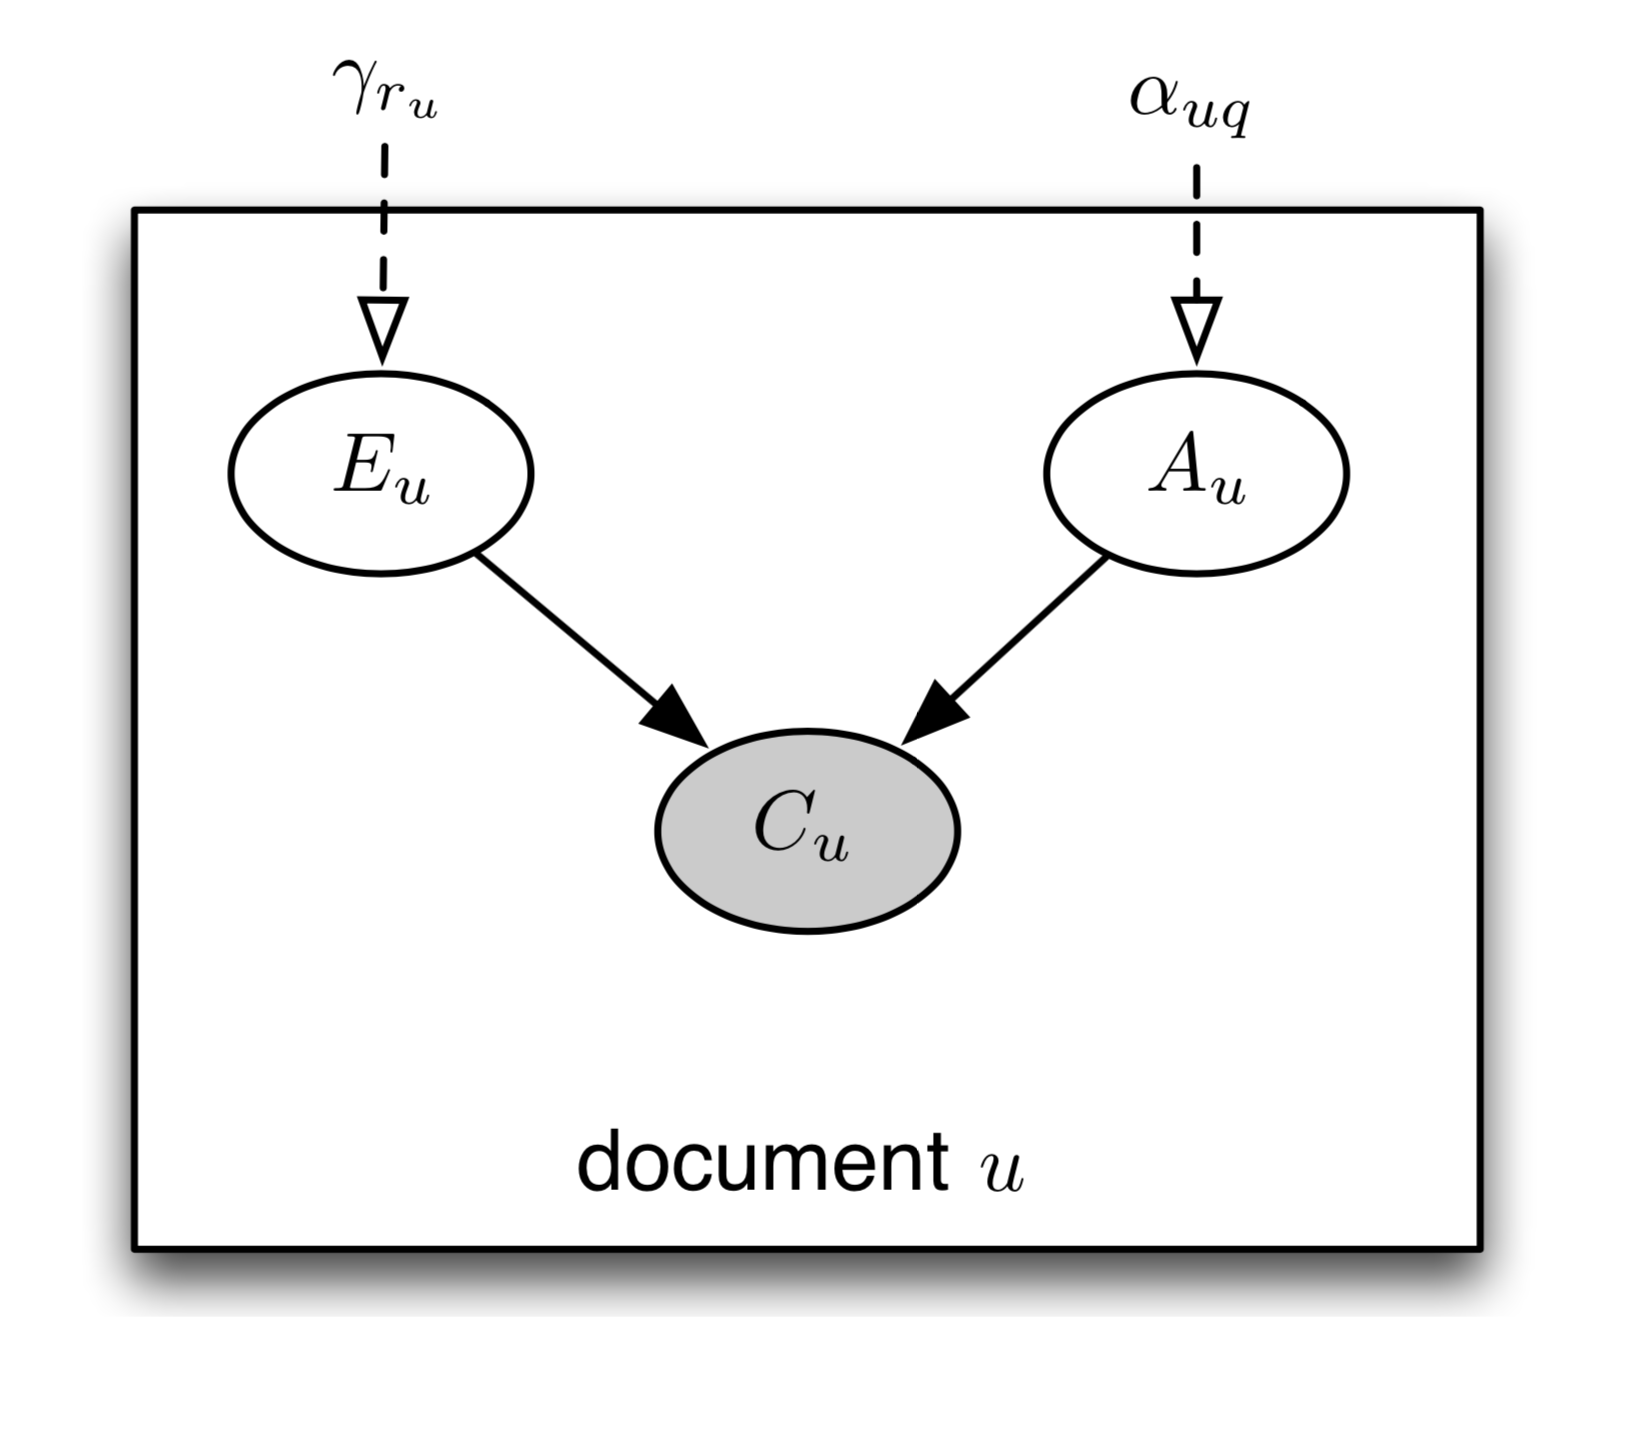
\includegraphics[width=0.25\textwidth]{figures/click_models_PBM_pgm.png}
		\caption{Probabilistic graphical model of parameters for PBM}
		\label{img:click_models_PBM_pgm}
	\end{figure}
	\item The examination models the position bias in user clicks while the attractiveness covers the document relevance
	\item \textit{Advantages}: Distinguishing between position bias and document relevance
	\item \textit{Disadvantages}: the Position-based model assumes that all clicks are independent of each other. Models that overcome this include:
	\begin{itemize}
		\item \textit{User browsing model (UBM)} - examination is also based on the rank of the previously clicked document $\implies$ $P(E_{r,r'}=1) = \gamma_{r,r'} $ ($n + n\cdot (n-1)/2$ parameters $\to$ 55 parameters for $n=10$)
		\item \textit{Cascade model} - see next section
	\end{itemize}
\end{itemize}
\subsection{Cascade model}
\begin{itemize}
	\item The cascade model assumes that the user scans the documents from top to bottom until he finds a relevant document and clicks
	\item Thus, the top document is always examined, while following documents are only examined if none of the previous ones were clicked
	\item The cascade model can be summarized in the equations:
	\begin{equation*}
		\begin{split}
			P(A_r = 1) & = \alpha_{u_r q}\\
			P(E_1 = 1) & = 1 \textit{\hspace{7mm} first element is always examined}\\
			P(E_r = 1|C_{r-1} = 1) & = 0 \textit{\hspace{7mm} stop if previous document is clicked}\\
			P(E_r = 1|E_{r-1} = 0) & = 0 \textit{\hspace{7mm} only examine if none of the documents before was clicked}\\
			P(E_r = 1|E_{r-1}=1, C_{r-1}=0) & = 1 \textit{\hspace{7mm} if no click was performed yet, examine next document}\\
		\end{split}
	\end{equation*}
	\item Therefore, the model has no parameters for examination and solely relies on attractiveness. The corresponding PGM is visualized in Figure~\ref{img:click_models_CM_pgm}
	\begin{figure}[ht]
		\centering
		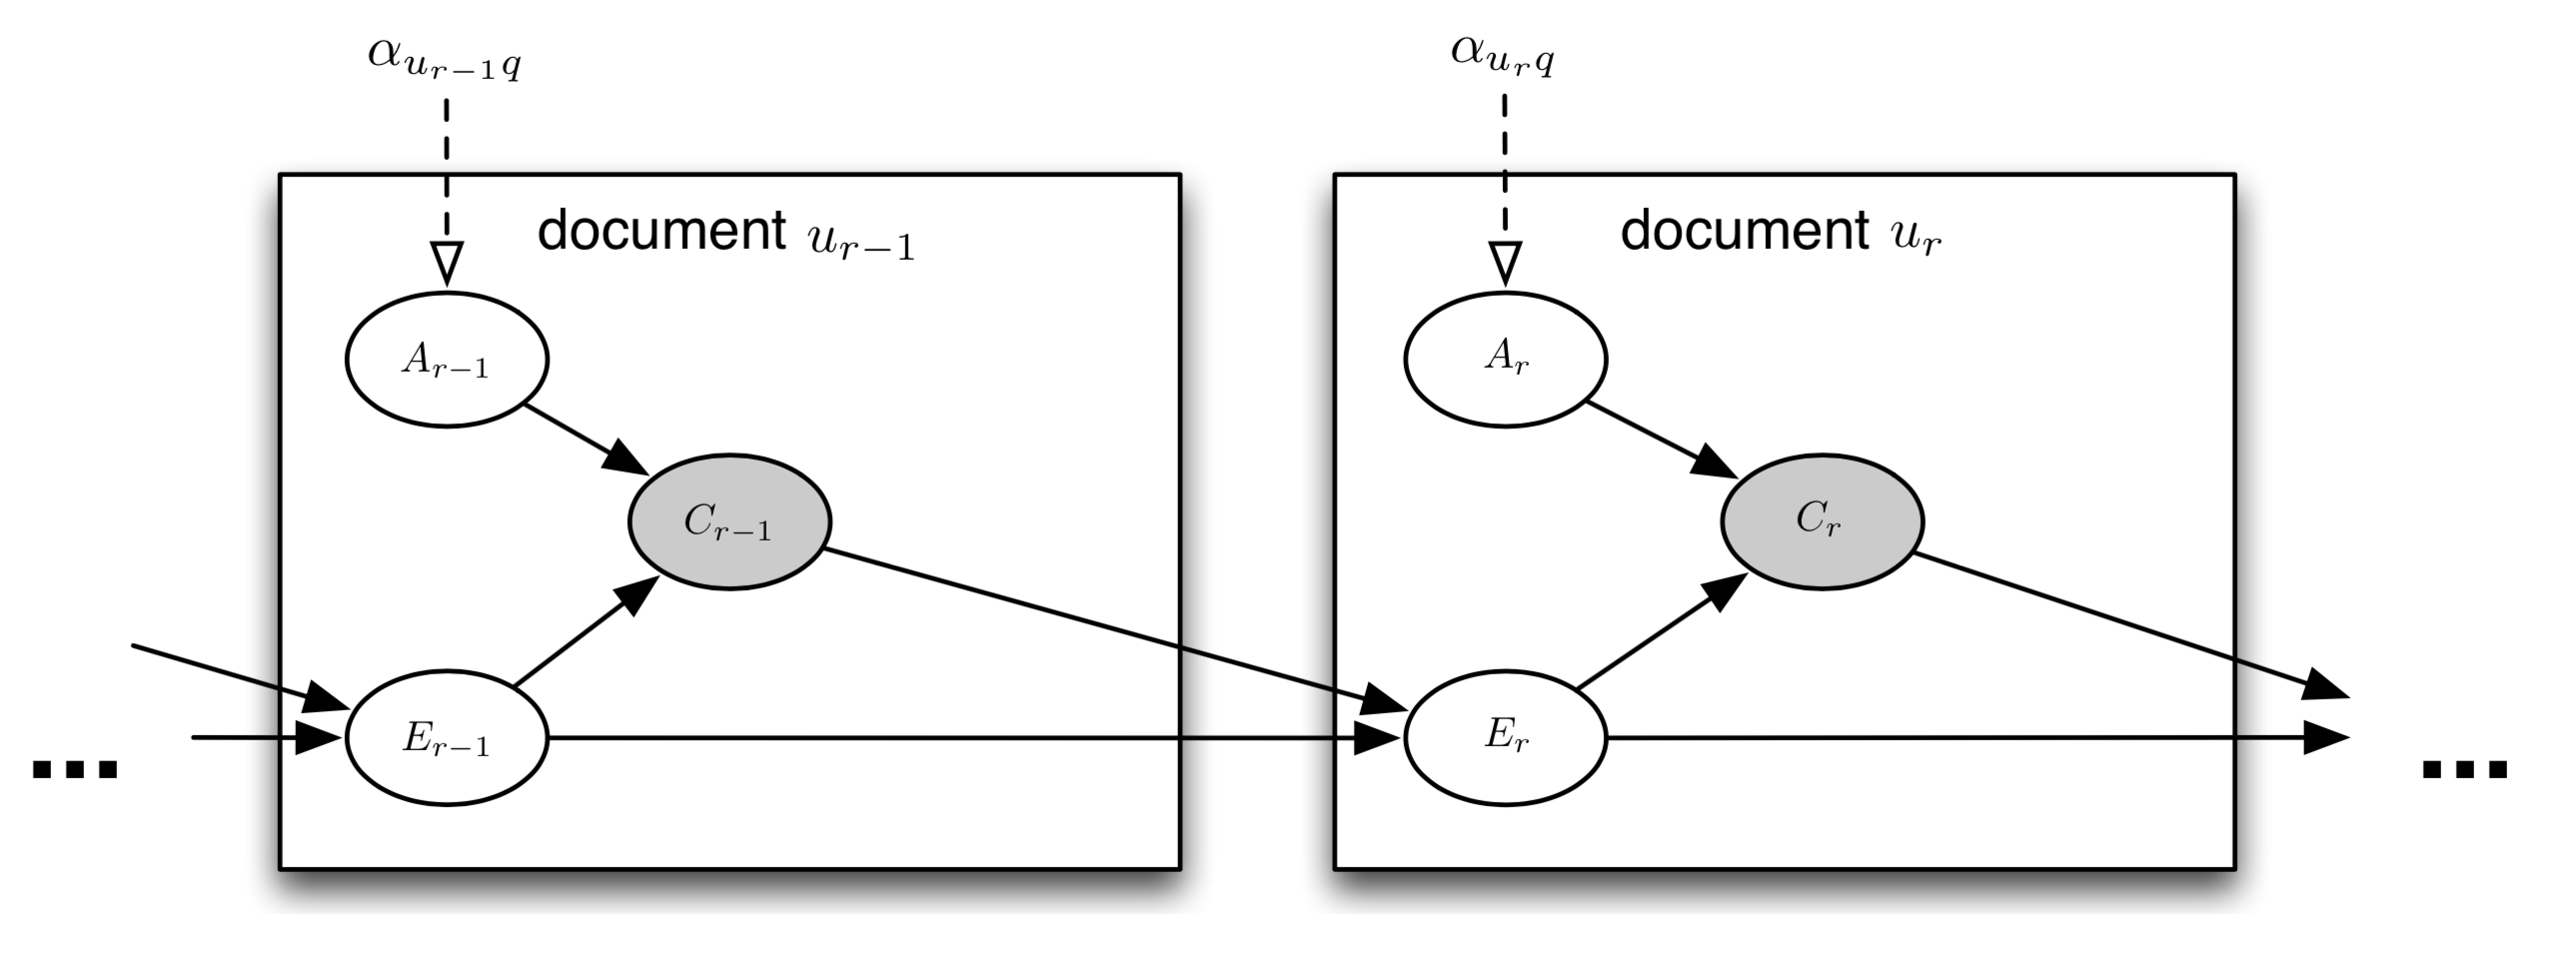
\includegraphics[width=0.5\textwidth]{figures/click_models_CM_pgm.png}
		\caption{Probabilistic graphical model of parameters for CM}
		\label{img:click_models_CM_pgm}
	\end{figure}
	\item \textit{Advantages}: Clicking on a document depends on previous decisions/documents
	\item \textit{Disadvantages}: No skips are allowed. Also, the cascade model only considers a single click $\implies$ Dynamic Bayesian Networks
\end{itemize}